\documentclass[10pt,journal,compsoc]{IEEEtran}

\usepackage{cite}
\usepackage[pdftex]{graphicx}

\begin{document}

\title{The past and future of visualization for computing in science and engineering}



\author{%
	Joao Comba, Daniel Weiskopf
	\IEEEcompsocitemizethanks{
	\IEEEcompsocthanksitem Joao Comba is at Universidade Federal do Rio Grande do Sul, Brazil\protect\\ 
	\IEEEcompsocthanksitem Daniel Weiskopf is at University of Stuttgart, Germany.
}}


\IEEEtitleabstractindextext{%
\begin{abstract}
The CiSE Visualization Corner (VizCorner) department  reflects the long-term and fruitful overlap between computer-based visualization and computational science and engineering. 
Looking into what the VizCorner has covered in the last decade, we identify current trends in visualization research,  and possible future developments for visualization in science and engineering.
\end{abstract}
}


% make the title area
\maketitle


\section{Retrospective of the VizCorner}

The CiSE Visualization Corner (VizCorner) department covers the breadth of visualization research and practice relevant to the readers of this magazine. 
As early as 1987, the Workshop on Visualization in Scientific Computing identified the need for visualization for the growing area of simulation-oriented science~\cite{NSFreport1987}. Visualization now plays a key role in visual data analysis and communication in science, engineering, and beyond. 
Organizing the papers from 2011 until now into themes highlights the focal areas of the VizCorner, 
and illustrates the breadth of visualization possibilities.


\subsection*{Multidimensional and multivariate data visualization}
% 4 papers:
% Paulovich, F., Silva, C., & Nonato, L. (2012). User-centered multidimensional projection techniques. Computing in Science and Engineering, 14(4), 74-81.
% Da Silva, R., Rauber, P., & Telea, A. (1. 9 2016). Beyond the third dimension: Visualizing high-dimensional data with projections. Computing in Science and Engineering, 18(5), 98-107.
% Doleisch, H., & Hauser, H. (3 2012). Interactive visual exploration and analysis of multivariate simulation data. Computing in Science and Engineering, 14(2), 70-76.
% Heinrich, J., & Weiskopf, D. (2015). Parallel coordinates for multidimensional data visualization: Basic concepts. Computing in Science and Engineering, 17(3), 70-76.

Multidimensional and multivariate data is almost omnipresent in computational science and engineering. 
Helmut Doleisch and Helwig Hauser~\cite{Doleisch2012} nicely showed how the combination of 2D and 3D visualization, flexible degree-of-interest definition, and interactive exploration lead to effective visual analysis of complex simulation data. They discussed how multiple simulation attributes from computational fluid dynamics can be visually analyzed. Figure~\ref{fig:simvis} shows a screenshot from their software system, illustrating how different visualization views are integrated in order to support a user-oriented exploration and analysis process.

\begin{figure*}
    \begin{center}    
        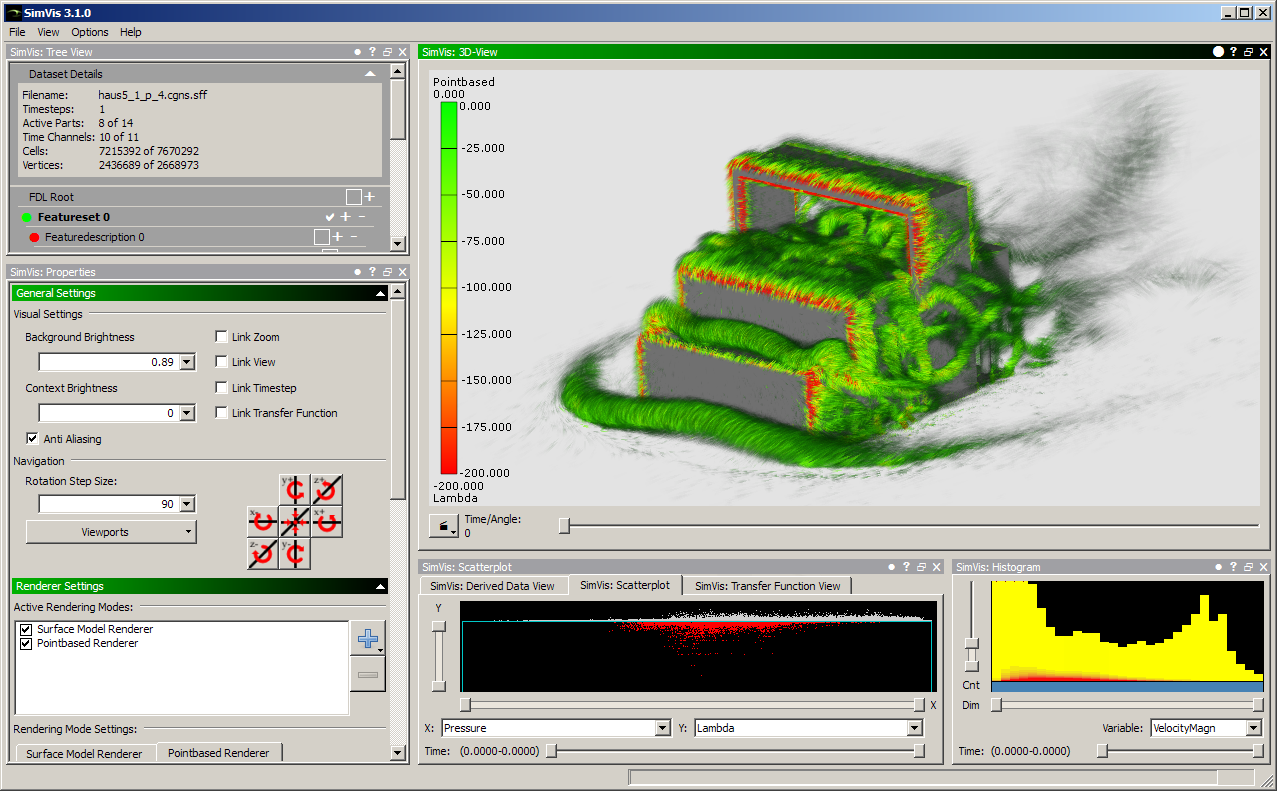
\includegraphics[width=0.9\textwidth]{simvis.png}
        \caption{Example of multivariate data visualization with the SimVis system. This screenshot shows the windflow around a building, where turbulent parts are emphasized using a vortex detection method. Image: \copyright{} 2012 IEEE, reprinted from Doleisch and Hauser~\cite{Doleisch2012}.
  \label{fig:simvis}}        
    \end{center}
\end{figure*}

The VizCorner has also covered projection techniques that reduce multidimensional data to 2D data for visualization purposes or methods that show multiple data dimensions simultaneously via parallel coordinates. Papers in this category often include generic visualizations that can be useful in many areas of science and engineering.

\subsubsection*{Flow visualization}
% 3+1 papers:
%Netzel, R., & Weiskopf, D. (2013). Texture-based flow visualization. Computing in Science and Engineering, 15(6), 96-102.
%Karch, G., Sadlo, F., Weiskopf, D., Hansen, C., Li, G., & Ertl, T. (2012). Dye-based flow visualization. Computing in Science and Engineering, 14(6), 80-86.
%Weinkauf, T., & Theisel, H. (2012). Flow visualization and analysis using streak and time lines. Computing in Science and Engineering, 14(5), 78-84.
% also in HCI: Englund, R., Palmerius, K., Hotz, I., & Ynnerman, A. (1. 5 2018). Touching Data: Enhancing Visual Exploration of Flow Data with Haptics. Computing in Science and Engineering, 20(3), 89-100.

A classic research area of scientific visualization, flow visualization considers input from flow simulation and experiments alike. Our pick from the VizCorner is by Grzegorz Karch and colleagues~\cite{Karch2012}, who described methods for high-quality computational flow visualization utilizing the metaphor of dye advection. Experimental flow visualization has a long tradition of dye-based observations. Its computational counterpart uses the same idea now in a computer-based visualization; see an example in Figure~\ref{fig:karman}. 

\begin{figure*}
	\begin{center}	
		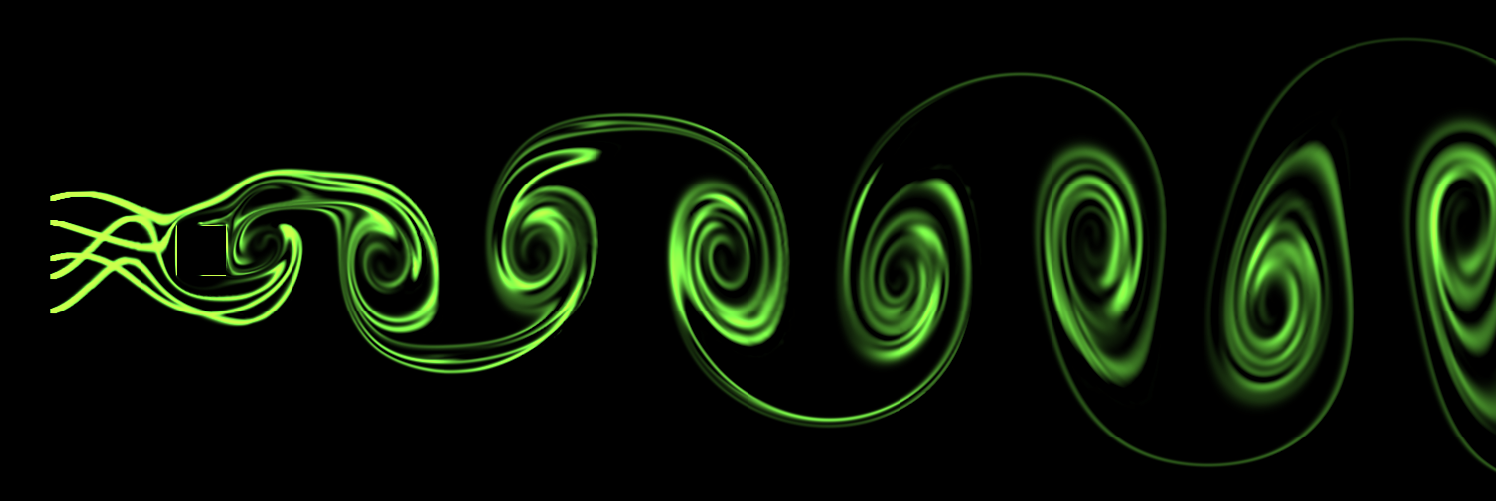
\includegraphics[width=0.9\textwidth]{karman_weno3.png}
		\caption{Computational dye advection applied to a 2D simulation of a von K{\'a}rm{\'a}n vortex street. Image: \copyright{} 2012 IEEE, reprinted from Karch et al.~\cite{Karch2012}.
  \label{fig:karman}}		
	\end{center}
\end{figure*}

The VizCorner has covered alternative visual representations of flow using textures or streak and timelines, 
and interaction techniques with haptics that let users virtually touch the data.

\subsubsection*{Human-computer interaction and storytelling}

%User perspective, user studies, HCI, perception (4)
%Kurzhals, K., Burch, M., Pfeiffer, T., & Weiskopf, D. (1. 9 2015). Eye Tracking in Computer-Based Visualization. Computing in Science and Engineering, 17(5), 64-71.
%Oliveira, M. (9 2013). Towards more accessible visualizations for color-vision-deficient individuals. Computing in Science and Engineering, 15(5), 80-87.
%Englund, R., Palmerius, K., Hotz, I., & Ynnerman, A. (1. 5 2018). Touching Data: Enhancing Visual Exploration of Flow Data with Haptics. Computing in Science and Engineering, 20(3), 89-100.
%Sauer, F., Neuroth, T., Chu, J., & Ma, K. (1. 11 2016). Audience-Targeted Design Considerations for Effective Scientific Storytelling. Computing in Science and Engineering, 18(6), 68-76.

Interaction plays an essential role in visualization, supporting scientists in exploring their simulation data. The VizCorner has highlighted new developments in eye tracking for interactive visualization or the role of human visual perception. Franz Sauer and colleagues~\cite{Sauer2016} went all the way to discussing visualization as a means of storytelling that can address a wide range of audiences, from domain scientists to general scientists to the public. They showcased an example of an interactive museum exhibit that visualized plankton populations for visitors; see Figure~\ref{fig:museum}.

\begin{figure*}
    \begin{center}    
        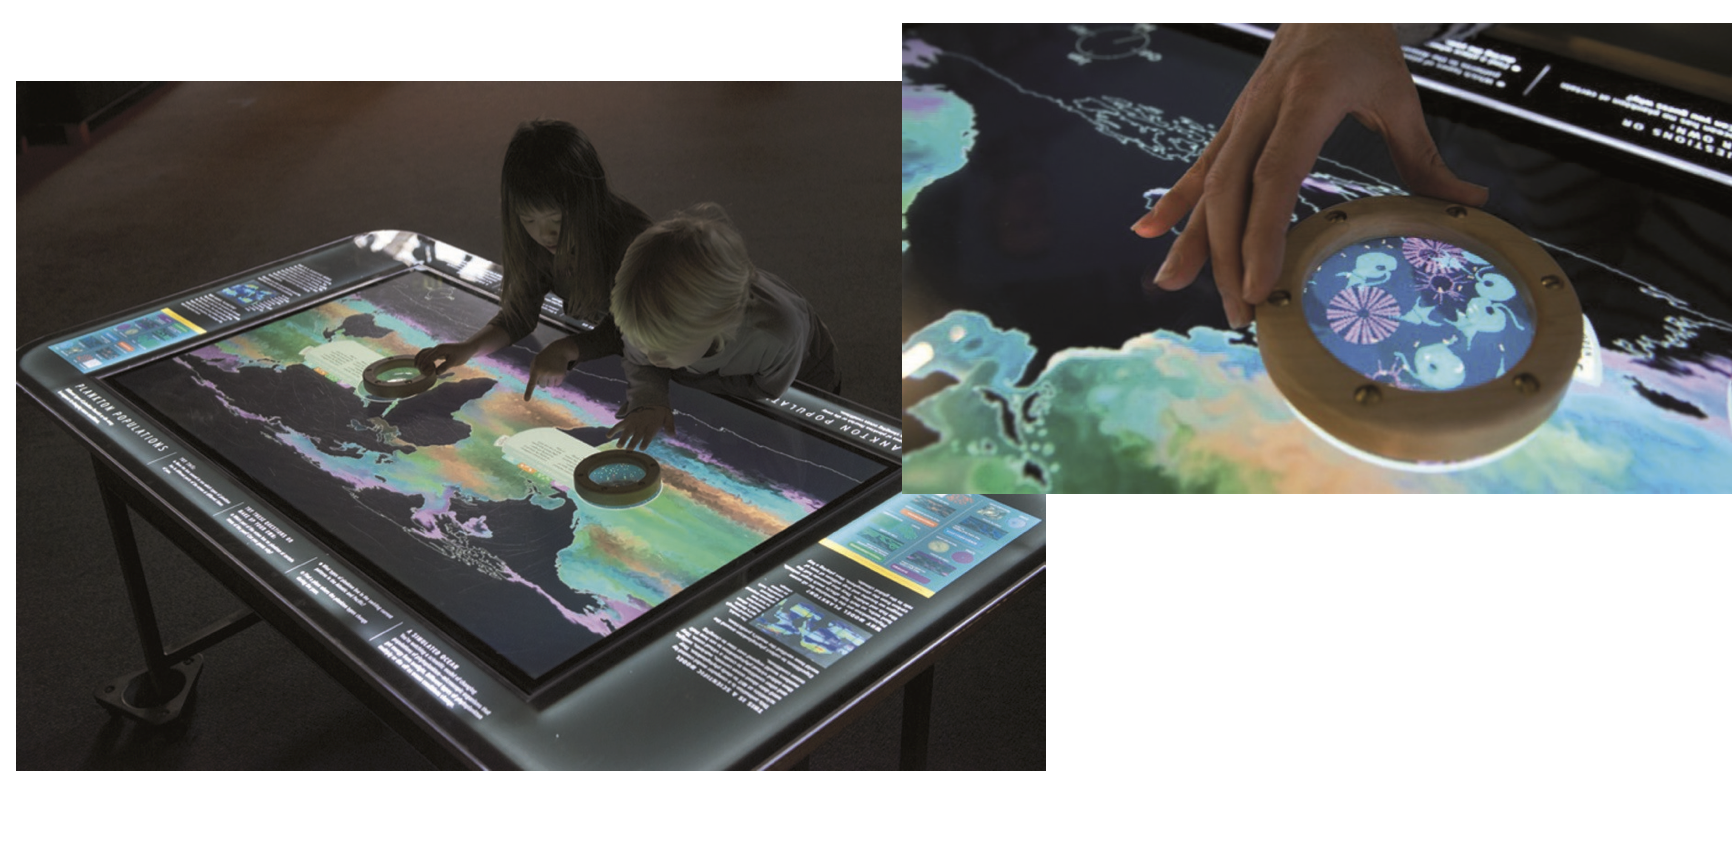
\includegraphics[width=\textwidth]{museum.png} 
        \caption{Interactive table with a plankton visualization. Image: \copyright{} 2016 IEEE, reprinted from Sauer et al.~\cite{Sauer2016}. 
  \label{fig:museum}}        
    \end{center}
\end{figure*}



\subsubsection*{Astronomy and astrophysics}

%Wenger, S., Ament, M., Steffen, W., Koning, N., Weiskopf, D., & Magnor, M. (5 2012). Interactive visualization and simulation of astronomical nebulae. Computing in Science and Engineering, 14(3), 78-87.
%Aragon-Calvo, M., & Subbarao, M. (1. 11 2015). A Flight through the Universe. Computing in Science and Engineering, 17(6), 96-102.
%Mller, T., & Weiskopf, D. (7 2011). Special-relativistic visualization. Computing in Science and Engineering, 13(4), 85-93.
%Muller, T., & Weiskopf, D. (11 2011). General-relativistic visualization. Computing in Science and Engineering, 13(6), 64-70.

The museum exhibit mentioned above links to other visualization activities for public outreach: 
Miguel Aragon-Calvo and Mark SubbaRao~\cite{Aragon-Calvo2015} described a virtual flight through the universe that addresses and balances scientific and artistic goals. They discussed how they adapted the virtual size of galaxies in order to address the issue of vast space between them in the visualization. Figure~\ref{fig:galaxies} shows a snapshot of a flight through the universe.

\begin{figure*}
    \begin{center}    
        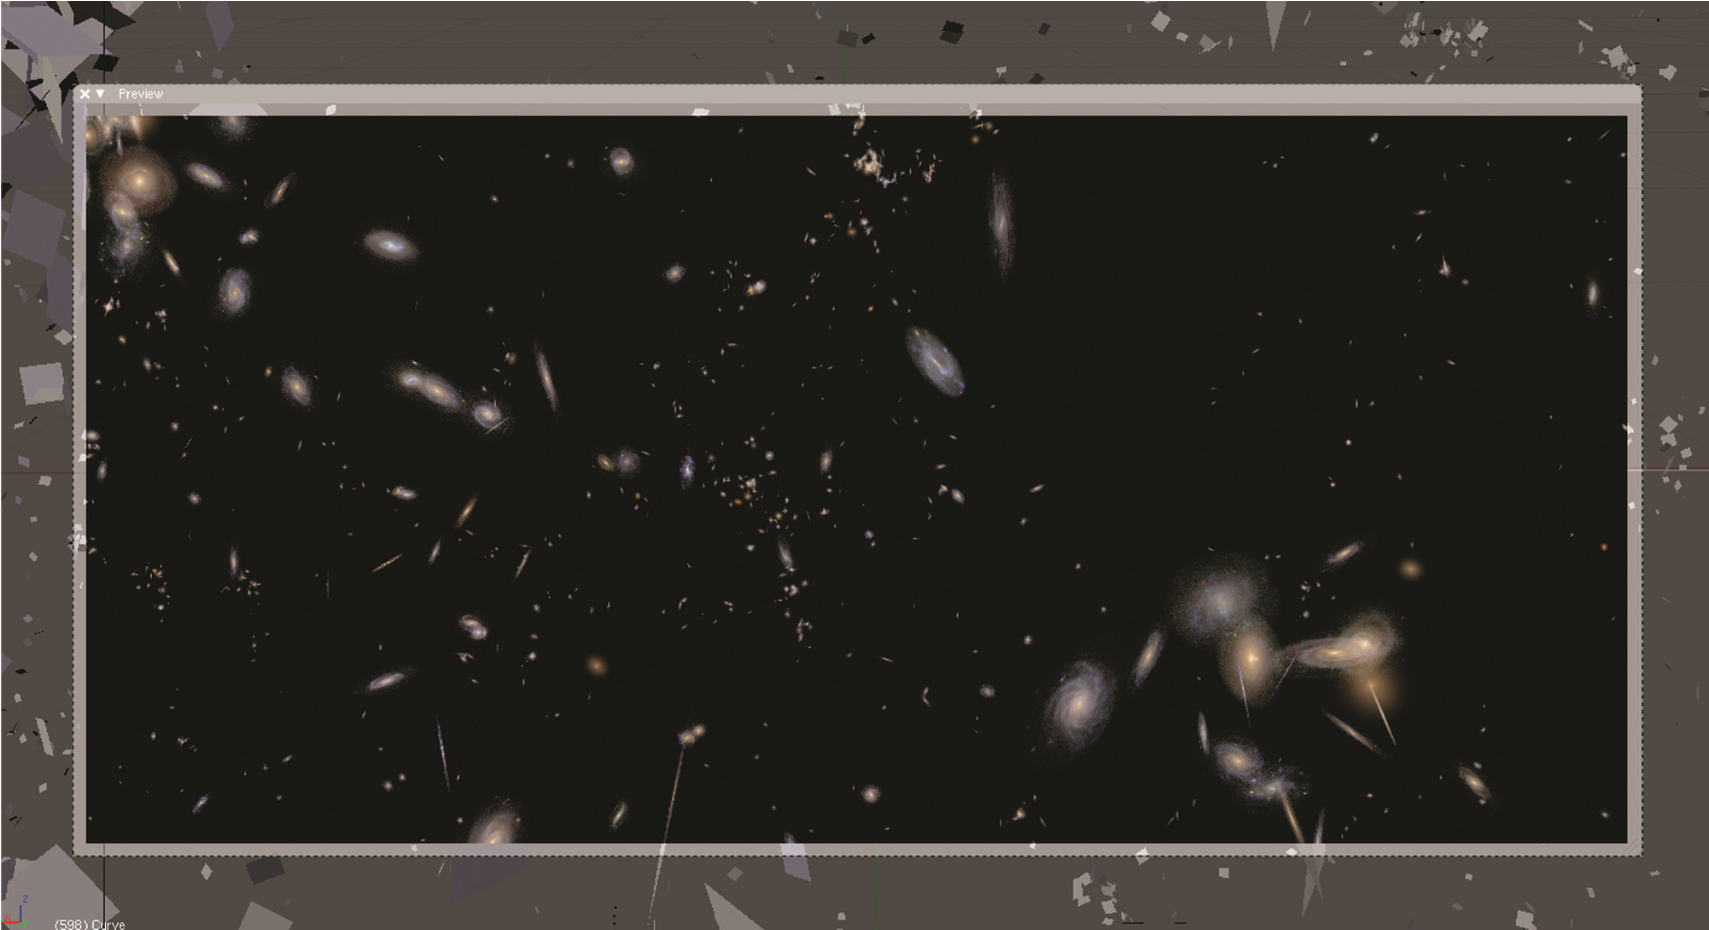
\includegraphics[width=0.9\textwidth]{galaxies.png}
        \caption{Virtual flight through the universe. 
 Image: \copyright{} 2015 IEEE, reprinted from Aragon-Calvo and SubbaRao~\cite{Aragon-Calvo2015}.
  \label{fig:galaxies}}        
    \end{center}
\end{figure*}

The VizCorner also looked into the issue of reconstructing 3D models of astronomical nebulae from 2D images along with the efficient volume rendering of such nebulae. Other papers discussed approaches to visualizing special relativity and general relativity. 


\subsubsection*{Other applications and visualization techniques}
%Salinet, J., Oliveira, G., Vanheusden, F., Comba, J., Ng, G., & Schlindwein, F. (2013). Visualizing intracardiac atrial fibrillation electrograms using spectral analysis. Computing in Science and Engineering, 15(2), 79-87.
%Santos, E., Poco, J., Wei, Y., Liu, S., Cook, B., Williams, D., & Silva, C. (2013). UV-CDAT: Analyzing climate datasets from a user's perspective. Computing in Science and Engineering, 15(1), 94-103.
%Michalski, M., Rieth, M., Kempf, A., & Krüger, J. (1. 11 2017). CoFlaVis: A visualization system for pulverized coal flames. Computing in Science and Engineering, 19(6), 72-78.

The VizCorner encompasses the breadth of possible applications of visualization. We have covered the visualization of climate data sets, simulation of coal combustion processes in the form of pulverized coal flames, or the visualization of intracardiac atrial fibrillation electrograms. Showing the full range of visualization applications from science to engineering to medical science, and the practical relevance of visualization, is among the goals of the VizCorner. 

With multidimensional and multivariate visualization, flow visualization, and human-computer interaction, we have already touched some relevant visualization themes that build a versatile foundation for many applications. The VizCorner is not restricted to these themes, and we have covered approaches to direct analytical support in visualization, advanced volume rendering, efficient parallel processing, mathematical modeling, or incorporating text in visualization.  %---showing the breadth in visualization methods relevant for science and engineering. 

%Text:
%Koch, S., Heimerl, F., & Ertl, T. (2013). Visual document retrieval: Supporting text search and analysis with visual analytics. Computing in Science and Engineering, 15(4), 66-74.
%Latif, S., & Beck, F. (1. 11 2018). Visually augmenting documents with data. Computing in Science and Engineering, 20(6).

%Unclassified:
%Ament, M., Weiskopf, D., & Dachsbacher, C. (1. 3 2016). Ambient volume illumination. Computing in Science and Engineering, 18(2), 90-97.
%Sadlo, F., Üffinger, M., Pagot, C., Osmari, D., Comba, J., Ertl, T., . . . Weiskopf, D. (5 2011). Visualization of cell-based higher-order fields. Computing in Science and Engineering, 13(3), 84-91.
%Vo, H., Comba, J., Geveci, B., & Silva, C. (9 2011). Streaming-enabled parallel data flow framework in the visualization toolkit. Computing in Science and Engineering, 13(5), 72-82.
%Andrienko, G., Andrienko, N., Bosch, H., Ertl, T., Fuchs, G., Jankowski, P., & Thom, D. (2013). Thematic patterns in georeferenced tweets through space-time visual analytics. Computing in Science and Engineering, 15(3), 72-82.



\subsubsection*{Summary and reflections}

This brief tour through past VizCorner articles shows the breadth of basic visualization techniques and the full range of exciting applications. We have seen some themes covered in more depth, such as flow visualization or multivariate data visualization---these are driven by typical visualization needs in science and engineering. The VizCorner also tries to bring in trends from the visualization research community that might have a more long-term impact on science and engineering. For example, advanced human-computer interaction techniques might eventually improve how engineers or scientists work with their visual-interactive tools. 

The VizCorner provided overviews of trends in visualization and the impact on computing in science and engineering, with synopsis of the 2011 and 2016 IEEE VIS Conferences (wwww.ieeevis.org), the premier venue for visualization research~\cite{Scheidegger2011,Comba2017}. Let us have a closer look at current trends in visualization research.


\section{Trends in visualization}

We want to share our perspective on what we see as important, ongoing trends. We adopt the point of view of visualization research as a whole, and address the particular interests for computing in science and engineering.

\subsection*{Interplay of artificial intelligence and visualization}

Artificial Intelligence (AI) techniques play a crucial role in recognition tasks. In particular, machine learning (ML) algorithms are efficient in pattern-recognition problems such as image classification, speech recognition, and sentiment analysis. Over the past years, we have seen an increasing intersection between ML and visualization with the popularity of Deep Learning (DL). Unlike classical ML algorithms, DL algorithms process sets of labeled samples using multiple layers to extract features automatically.
A common intersection between AI and visualization is related to the field of explainable AI, where we use visualization techniques to gain insights into the inner workings of DL neural networks. We have recently seen several works that describe techniques to interpret DL models~\cite{hohman2018visual,GARCIA2018}. Most approaches aim at understanding how features are perceived during the learning process, in which visualization techniques can offer insights to improve the process.

The complexity of DL architectures also benefits from visualization to identify which aspects of the network can be modified. Finally, the understanding of the inner working of a deep model, a process called training analysis, has also been drawing attention recently by including the human in the loop. Such techniques are being referred to as interactive visual machine learning (IVML). As the popularity of DL grows steadily, we foresee that visualization techniques will continue to play a crucial role in understanding and improving new approaches. 


\subsection*{Getting insights from data: visualization in data science}

Data is at the center of essential tasks in our society, such as decision-making, planning strategies, or process optimizations, and of course, also in data-driven science and engineering. 
Extracting insights from data is challenging because data is often massive, heterogeneous, subject to errors, and comes in a streaming fashion. Along with other fields such as applied mathematics, statistics, ML (see above), and computational modeling, visualization plays a fundamental part in data analysis. Urban data is a good example that can benefit from visualization techniques, such as spatio-temporal representations of data~\cite{Doraiswamy2018}. Several works describe ways to understand mobility patterns in cities from their fleet of taxis, trains, or bike-sharing systems. 
%Sports is another source of data that significantly benefit from visualization techniques. 
%Several approaches use visualization to understand soccer, tennis, and baseball matches, among other sports~\cite{perin2018}. 
Another example is social media. Visualization techniques are being used to display and explore social networks and their flow of information diffusion, or even explore the textual content shared among users~\cite{Chen2017}. Visual text analysis, which combines visualization along with other areas such as data mining, natural language processing, and machine learning, offers great ways to extract insights from social media. In all these examples, we see how visualization techniques allow the extraction of insights from large, heterogeneous, and unstructured data. In science and engineering, we observe a growing need for this type of data and similar needs for insights. 

%{\bf TODO: Link to science and engineering?! Especially since the last few lines are not really on CiSE topics.}

\subsection*{Integration of VIS subfields}

IEEE VIS has been structured around its three main conferences: the IEEE Conference on Visual Analytics Science and Technology (VAST), the IEEE Conference on Information Visualization (InfoVis), and the IEEE Conference on Scientific Visualization (SciVis). 
Scientific visualization primarily considers data from scientific applications, i.e., it is the natural link to computing in science and engineering. It usually deals with data with a given spatial embedding such as 3D scalar or vector fields. Information visualization typically works with data lacking a given spatial mapping; for example, the visualization of networks or high-dimensional data. Melanie Tory and Torsten M{\"o}ller provide details on spatial and non-spatial visualization \cite{ToryM04}. Finally, visual analytics often includes ML techniques for improved data analysis and addresses the challenges of data science.

The separation of the three subfields is not so clear in practice. For example, multidimensional or multivariate data is highly interesting in science and engineering and, therefore, appropriate visualizations will likely include both SciVis and InfoVis techniques. We have seen a lot of exciting papers that combine techniques from the subfields of VIS; these are particularly interesting for computing in science and engineering. 
IEEE VIS reflects this trend toward combined techniques by integrating the VAST, InfoVis, and SciVis Conferences, according to the results of a restructuring process (http://ieeevis.org/governance/restructuring).

Besides this integration, we have also been witnessing visualization as a growing and maturing field. Fundamental and long-standing research challenges are still being addressed, but now on a more refined and advanced level. As an example that is particularly relevant for computing in science and engineering, there is ongoing research on making visualization useful for applications in high-performance computing (HPC), by exploiting in-situ visualization integrated into the HPC environment or developing efficient, parallel visualization techniques. Another ongoing topic targets improved mathematical methods for visualization, for example, relying on topological techniques or uncertainty quantification. 

In summary, we expect that the integration of the subfields of visualization will continue and deliver improved visualization systems. We also see ongoing research in several of these subfields that are relevant for applications in science and engineering.


\subsection*{Visualization and human-computer interaction}

We have also been witnessing an increasingly strong link between visualization and human-computer interaction (HCI) research. One theme of our retrospective addresses HCI from the visualization perspective. With interactive data exploration, interaction techniques play an important role in visualization, with a large number of papers at IEEE VIS. Visualization has also become interesting for HCI research. This is reflected by the fact that the leading HCI conference---ACM CHI (https://chi.acm.org)---now includes a separate subcommittee for visualization. This link strengthens the human-centered perspective on visualization.
It is the right way of addressing the long-standing and challenging issue of evaluating visualization approaches from the user's perspective. For example, the series of BELIV Workshops (https://beliv-workshop.github.io/) targets this issue. While these HCI and user-based evaluation problems are primarily interesting for basic visualization research, we expect that improved interactive visualization will eventually impact any visualization application, including ones in science and engineering.


\section{Conclusion}

Our retrospective of the VizCorner in the last ten years and the outlook on trends show that visualization is a thriving and evolving research field with many interesting connections to computing in science and engineering. With this paper, the tenure of one of the current co-editors (Daniel Weiskopf) will end. 
I, Daniel, have been serving in this role since 2011, and it has been a great pleasure working for the VizCorner. Thanks to all readers and authors of the VizCorner, and special thanks to my former co-editor Claudio Silva, my current co-editor Joao Comba, and the whole CiSE team!

The VizCorner will continue with a new incoming co-editor joining Joao, who will help us to refresh the topics covered in the department. We look forward to bringing interesting new articles in the years to come.

%TODO: Joao: anything on call for papers? Future plans?
%With visualization thriving as an important topic for computing in science ...

\bibliographystyle{IEEEtran}
\bibliography{./refs}

\bigskip

\textbf{Joao Comba} is a full professor of computer science at UFRGS, Brazil. His research interests include visual analytics, data science, information visualization, geometric algorithms, spatial data structures and high-performance computing. Joao Comba received a Ph.D. in computer science from Stanford University, USA. Contact him at comba@inf.ufrgs.br.


\textbf{Daniel Weiskopf} is a professor of computer science at the University of Stuttgart, Germany. His research interests include visualization, visual analytics, eye tracking, computer graphics, and special and general relativity. Weiskopf received a Dr. rer. nat. (PhD) in physics from the University of T\"ubingen, Germany. Contact him at weiskopf@visus.uni-stuttgart.de.



\end{document}